\chapter{Diseño del sistema.}
\label{cap: capitulo_4}

En este capítulo vamos a detallar cómo hemos concebido la solución a los requisitos \textit{software}, teniendo en cuenta los correspondientes al \textit{hardware} y a partir de los elementos que hemos detallado en el capítulo anterior.

\section{Planteamiento}

Como idea más abstracta, el \textit{software} que tenemos que diseñar consiste en un reproductor de archivos \textit{MIDI}, que recibe el fichero y lo envía a la \textit{PCB} a través del \textit{GPIO}. Por supuesto, la reproducción estará controlada por el usuario:

\smallskip

\begin{figure}[H]
	\noindent \begin{centering}
		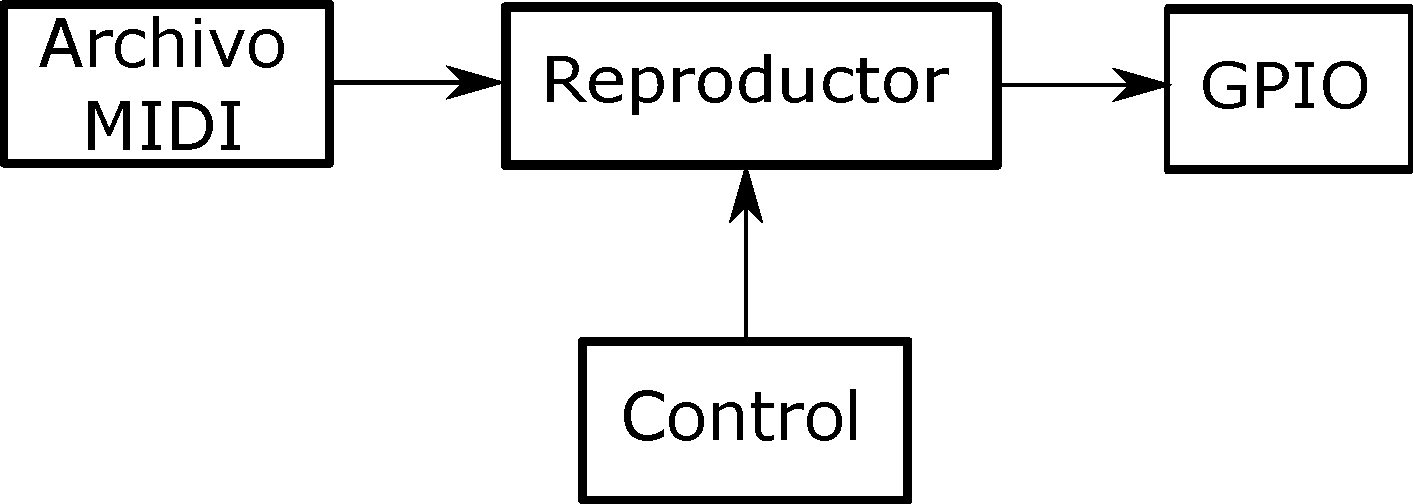
\includegraphics[width=\linewidth/2]{capitulo4/figura4_idea}
		\par\end{centering}
	\smallskip
	\caption{\label{fig:figura4_idea} Planteamiento inicial.}
\end{figure} 

\smallskip

Luego, dividiremos el sistema en cuatro grandes bloques. Respecto al de control, se requiere varias formas de acceder al sistema:

\begin{enumerate}
	\item Un \textit{software} controlador principal, que cubra todos los casos de uso, y sea fácil de instalar y utilizar, con preferencia de que sea multiplataforma.
	
	\item Un mando a distancia, que altere la reproducción.
	
	\item Un control reducido empotrado en la \textit{PCB}.
\end{enumerate}

Atendiendo a los requisitos del primer controlador y a las prestaciones del \textit{Raspberry Pi}, y con objeto de eliminar la necesidad de instalar y mantener aplicaciones en otro sistema, decidimos enfocar la solución como una interfaz \textit{web} con un servidor alojado en el \textit{Raspberry Pi}. De esta forma podemos llegar fácilmente a cualquier sistema operativo de escritorio, incluso es fácilmente adaptable a dispositivos móviles.

Sin embargo, el reproductor no puede funcionar dentro de un servidor \textit{web}, ya que éstos atienden peticiones sin estado, y se cierran automáticamente después de devolver la información. Por ello, vamos a diseñar el reproductor como un \textit{demonio} de \textit{Linux}, junto con sus módulos auxiliares.

En último lugar, necesitamos almacenar información de los archivos \textit{MIDI}, listas de reproducción y asignaciones del mando en memoria persistente. Una base de datos nos permitiría guardar toda esa información de manera estructurada y coherente, además de ser fácilmente accesible por todos los componentes del sistema.

\section{Demonio del reproductor}

Un demonio ---\textit{daemon}--- es un proceso que se ejecuta en segundo plano en la fase de arranque del sistema operativo, y no interactúa directamente con el usuario, sino que se comunica con otros procesos a través de herramientas proporcionadas por el sistema operativo.

Este programa será el núcleo de nuestro sistema, y ofrecerá las siguientes vías para comunicarse:

\begin{enumerate}
	\item Un \textit{socket} local de \textit{Linux}. Será usado principalmente por la interfaz \textit{web}, pero es una forma flexible y eficiente para que lo hagan más aplicaciones.
	
	\item El puerto en serie (\textit{UART}) del \textit{Raspberry Pi}, para recibir órdenes del mando.
	
	\item Los pines del \textit{GPIO} correspondientes al codificador rotatorio y el \textit{LCD}, para la interfaz reducida.
\end{enumerate}

Así, el esquema de uso de los distintos componentes queda así:

\smallskip

\begin{figure}[H]
	\noindent \begin{centering}
		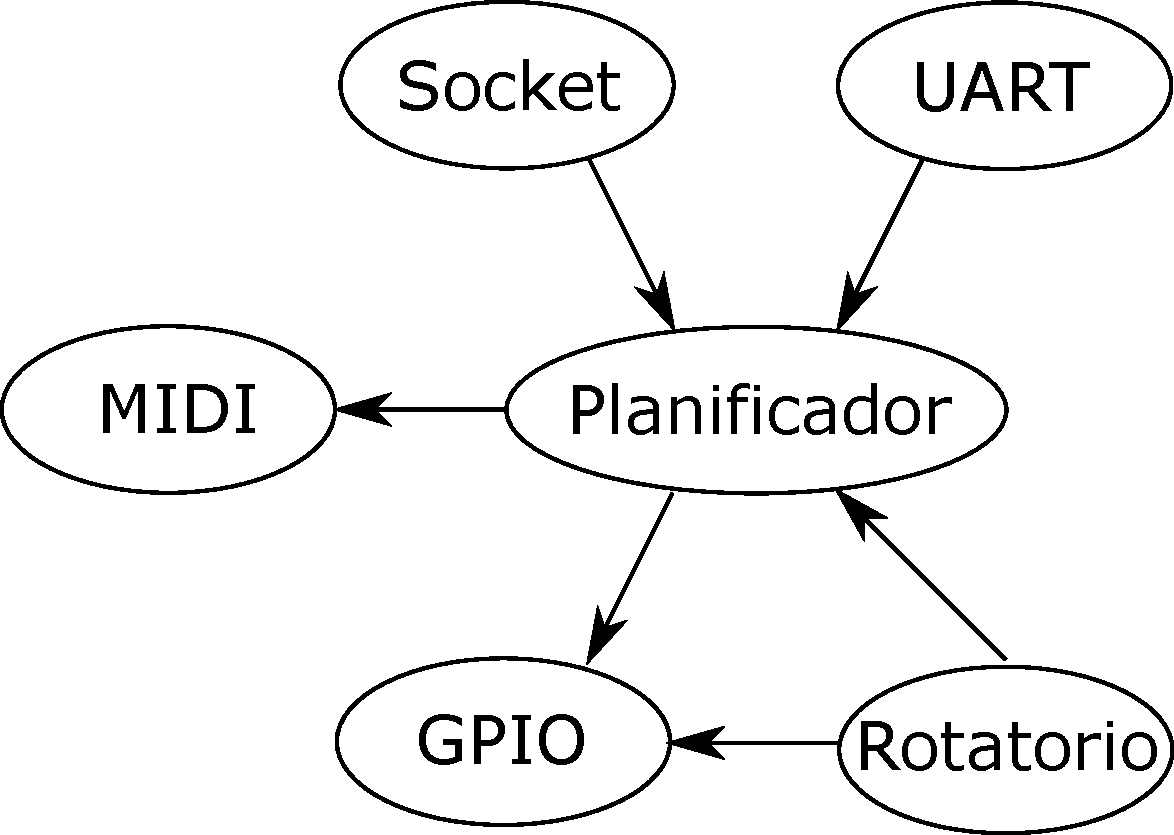
\includegraphics[width=\linewidth/2]{capitulo4/figura4_daemon}
		\par\end{centering}
	\smallskip
	\caption{\label{fig:figura4_daemon} Diagrama de uso entre los componentes del reproductor.}
\end{figure} 

\smallskip

\subsection{Descodificador de MIDI}

Como hemos detallado más arriba, el formato \textit{MIDI} expone los eventos de control en orden temporal, clasificados por pistas, habitualmente simultáneas. Debemos proporcionar una estructura de datos que permita mantener cada archivo a reproducir en memoria y facilitar el acceso individual a cada pista.

Concebimos la estructura de datos como un conjunto de listas enlazadas de eventos. El tamaño de los eventos normales es constante, sin embargo, los meta-eventos extienden la semántica con una cadena de datos.

\subsubsection{Estructura \textit{midifile\_t}}

Define un archivo \textit{MIDI}. Sus campos son:

\begin{description}
	\item[format : \textit{enum}] Formato del archivo. Puede tener los siguientes valores enumerados:
	
	\begin{description}
		\item[SINGLE\_TRACK] Una sola pista.
		\item[MULTIPLE\_SIMULTANEOUS] Varias pistas, simultáneas.
		\item[MULTIPLE\_INDEPENDENT] Varias pistas, independientes.
	\end{description}
	
	\item[ntracks : \textit{word}] Número de pistas.
	
	\item[division : \textit{enum}] Unidad de medida de la división de tiempo:
	
	\begin{description}
		\item[TICKS\ PER\ BEAT] La división se especifica en \textit{ticks}/\quarternote.
		\item[FRAMES\_PER\_SECOND] La división se especifica en \textit{ticks/fotograma}.
	\end{description}
	
	\item[tracks : \textit{array(midievent\_t)}] Conjunto de listas de eventos; cada lista corresponde a una pista.

\end{description}

\subsubsection{Estructura midievent\_t}

Define un evento MIDI.

\begin{description}
	\item[delta : \textit{dword}] Separación temporal respecto al evento anterior.
	\item[type : \textit{enum}] Tipo de evento. Se enumeran en el capítulo anterior.
	\item[param1 : \textit{byte}] Valor del primer parámetro, dependiendo del tipo de evento.
	\item[param2 : \textit{byte}] Valor del segundo parámetro, dependiendo del tipo de evento.
	\item[metaevent : \textit{metaevent\_t}] Información del metaevento, si procede.
	\item[next : \textit{midievent\_t}] Evento siguiente, si procede.
\end{description}

\subsubsection{Estructura \textit{metaevent\_t}}

Define un meta-evento.

\begin{description}
	\item[type : \textit{emum}] Tipo de metaevento. Se enumeran en el capítulo anterior.
	\item[length : \textit{dword}] Longitud de la cadena de datos, en \textit{bytes}.
	\item[data : \textit{string}] Cadena de datos correspondientes al meta-evento.
\end{description}

\subsubsection{Funciones}

\begin{description}[style=nextline]
	\item[midifile\_init (score, path) : \textit{int}] 
	Lee un archivo MIDI e inicializa la estructura recibida. 
	
	\begin{description}
		\item[score : \textit{midifile\_t}] Archivo \textit{MIDI} sin inicializar.
		\item[path : \textit{string}] Ruta del fichero a leer.
	\end{description}
	
	Devuelve 0 en caso de éxito, o -1 en caso de error.
	
	\item[midifile\_destroy (file)] 
	Elimina una estructura y libera su memoria.
	
	\begin{description}
		\item[file : \textit{midifile\_t}] Archivo \textit{MIDI}.
	\end{description}
	
	\item[midifile\_duration (file) : \textit{dword}] 
	Obtener la duración de una pieza.
	
	\begin{description}
		\item[file : \textit{midifile\_t}] Archivo \textit{MIDI}.
	\end{description}
	
	Devuelve la duración de la pieza, en \textit{segundos}.
	
	\item[metaevent\_tempo (event) : \textit{dword}] 
	Obtener el \textit{tempo} de la pieza.
	
	\begin{description}
		\item[event : \textit{metaevent\_t}] Meta-vento.
	\end{description}
	
	Devuelve el \textit{tempo} de la pieza en \textit{$\mu s$/\quarternote}.
	
\end{description}

\subsection{Control por socket}

Un \textit{socket} un mecanismo de comunicación inter-proceso ---\textit{IPC (inter-process communication)} que proporciona \textit{Linux} y enviar y recibir datagramas en modo \textit{duplex}, bien dentro de la misma máquina (\textit{socket} local) o en una red (\textit{socket} de Internet).

Vamos a crear un \textit{socket} local, accesible desde el sistema de archivos de \textit{Linux}, que escuche peticiones de los clientes que se conecten, utilizando una interfaz basada en lenguaje natural, que explicaremos a continuación.

Las funciones diseñadas son las siguientes:

\begin{description}[style=nextline]
	\item[socket\_init (uid, gid) : \textit{dword}]
	Inicializar el \textit{socket} con el ID de usuario y grupo indicados.
	
	\begin{description}
		\item[uid : \textit{dword}] ID de usuario en Linux.
		\item[gid : \textit{dword}] ID de grupo en Linux.
	\end{description}
	
	Devuelve 0 en caso de éxito y -1 en caso de error.
	
	\item[socket\_destroy ()]
	Cierra el \textit{socket}.
	
	\item[socket\_loop ()]
	Despliega una hebra con un bucle de escucha y atiende las peticiones.
	
\end{description}

\subsubsection{Lenguaje de la interfaz}

El \textit{socket} reconocerá y ejecutará una serie de órdenes, emitiendo siempre una respuesta:

\begin{description}
	\item[PLAY <archivo> [ <archivo>*]] Reproducir una lista de archivos MIDI, indicando las rutas completa, separadas por espacios. Respuesta:
	
	\begin{description}
		\item[OK] en caso de éxito.
		\item[ERROR] en caso de error o estar en modo Ingeniería.
	\end{description}
	
	\item[PLAYLOOP <archivo> [ <archivo>*]] Reproducir en bucle una lista de archivos MIDI, indicando las rutas completa, separadas por espacios. Respuesta:
	
	\begin{description}
		\item[OK] en caso de éxito.
		\item[ERROR] en caso de error o estar en modo Ingeniería.
	\end{description}
	
	\item[PAUSE] Pausar la reproducción. Silencia las notas pero manteniendo el estado. Respuesta:
	
	\begin{description}
		\item[OK] en caso de éxito.
		\item[ERROR] en caso de error, como estar detenido, o en modo Ingeniería.
	\end{description}
	
	\item[RESUME] Reanuda la reproducción en el punto en que se pausó. Respuesta:
	
	\begin{description}
		\item[OK] en caso de éxito.
		\item[ERROR] en caso de error, como no estar pausado, o en modo Ingeniería.
	\end{description}
	
	\item[STOP] Detiene completamente la reproducción y libera la lista de reproducción. Respuesta:
	
	\begin{description}
		\item[OK] en caso de éxito.
		\item[ERROR] en caso de error o estar en modo Ingeniería.
	\end{description}
	
	\item[STATUS] Consulta el estado del reproductor. Respuesta:
	
	\begin{description}
		\item[PLAYING <archivo>] Reproduciendo el archivo cuya ruta absoluta se especifica.
		\item[PAUSED <archivo>] Pausado en un punto del archivo cuya ruta se indica.
		\item[STOPPED] Detenido. Es el estado inicial.
		\item[ENGINEER] En modo Ingeniería. No se puede reproducir nada hasta desbloquearse.
	\end{description}
	
\end{description}

\subsection{Control del mando}

Como hemos indicado en el capítulo anterior, el receptor del mando a distancia está conectado al \textit{Raspberry Pi} a través de los pines correspondientes al dispositivo \textit{UART} ---\textit{Universal Asynchronus Receiver-Transmiter}---, que controla los puertos serie.

Este módulo tiene una topología análoga al control por \textit{socket}, tan solo cambia el origen y la forma de entrada de los datos. Establecerá una comunicación con el puerto serie e iniciará un bucle de escucha. La sintaxis del mensaje, como ya sabemos, es:

\begin{center}
	<Nº serie (7 \textit{bytes})> <Botón (1 \textit{byte})> <CRLF>
\end{center}

De esta forma, el servicio tan solo debe verificar el nº de serie y ejecutar la orden correspondiente.

Las funciones correspondientes a este módulo son las siguientes:

\begin{description}[style=nextline]
	\item[uart\_init () : \textit{dword}]
	Establece comunicación con el puerto serie.
	
	Devuelve 0 en caso de éxito y -1 en caso de error.
	
	\item[uart\_destroy ()]
	Cierra la comunicación.
	
	\item[uart\_loop ()]
	Despliega una hebra con un bucle de escucha y ejecuta las órdenes.
	
\end{description}

\subsubsection{Comunicación con la base de datos}

La información relativa a la lista de reproducción asignada a un botón, así como la lista de partituras correspondientes, residirán en una base de datos, que definiremos próximamente. Así, enmarcaremos un nuevo módulo dedicado a consultar la información requerida, mediante las siguientes funciones:

\begin{description}[style=nextline]
	\item[db\_init () : \textit{dword}]
	Inicia la comunicación con el gestor de bases de datos. Devuelve 0 en caso de éxito y -1 en caso de error.
	
	\item[db\_destroy ()]
	Cierra la comunicación.
	
	\item[db\_query (scores, idshortcut) : \textit{dword}]
	Realiza la consulta mencionada, asignando a \textit{scores} la lista de piezas a reproducir.
	
	\begin{description}
		\item[scores : \textit{array(string)}] Lista de rutas a las piezas.
		\item[idshortcut : \textit{dword}] ID del botón que se ha pulsado en el mando.
	\end{description}
	
	Devuelve el número de piezas asignadas (pudiendo ser 0), o -1 en caso de error.
	
\end{description}

\subsection{Planificador}

El planificador es la pieza principal del reproductor. Recibe las órdenes de los controladores y la lista de partituras a ejecutar. Una a una las lee con ayuda del módulo \textit{MIDI} y planifica los eventos de todas las pistas para lanzarlos a la salida en el momento necesario.

Al igual que otros módulos, utiliza una hebra para reproducir los archivos, pero en este caso es una hebra dinámica, que podrá ser iniciada, pausada y detenida por el resto de procesos, por lo que hay que tener en cuenta los problemas de concurrencia para garantizar la consistencia del sistema.

La interfaz que el planificador ofrece es la que sigue:

\begin{description}[style=nextline]
	\item[player\_start (playlist, n, loop) : \textit{dword}]
	Inicia la reproducción de una lista de archivos. Si ya estaba reproduciendo una lista, primero detiene la reproducción y elimina la lista antigua.
	
	\begin{description}
		\item[playlist : \textit{array(string)}] Lista de rutas absolutas a los archivos que queremos reproducir.
		\item[n : \textit{dword}] Número de piezas que se han transmitido en el parámetro anterior.
		\item[loop : \textit{bool}] Utilizar (1) o no (0) reproducción en bucle.
	\end{description}
	
	Devuelve 0 en caso de éxito o -1 en caso de error.
	
	\item[player\_pause () : \textit{dword}]
	Pausa la reproducción, si estaba activa. Devuelve 0 en caso de éxito o -1 en caso de error.
	
	\item[player\_stop () : \textit{dword}]
	Detiene completamente la reproducción, si estaba activa o pausada. Si estaba parado, no hace nada. Devuelve 0 en caso de éxito o -1 en caso de error.
	
	\item[player\_wait () : \textit{dword}]
	Espera a que el reproductor se detenga. Solo tiene sentido llamarla en caso de no estar reproduciendo en bucle. Devuelve 0 en caso de éxito o -1 en caso de error.
	
	\item[player\_state (file) : \textit{enum}]
	Indica el estado actual del planificador. Tales estados se detallan en el apartado siguiente.
	
	\begin{description}
		\item[file : \textit{array(string)}] Es un parámetro de salida, sobre él se escribe el nombre del archivo que se estaba reproduciendo. Solo es válido si el reproductor está activo o en pausa.
	\end{description}
	
	Devuelve el estado actual del reproductor, a saber entre los estados contemplados en la máquina.
	
	\item[player\_engineer\_enter () : \textit{dword}]
	Detiene el reproductor, bloquea el planificador y entra en modo Ingeniería. Devuelve 0 en caso de éxito o -1 en caso de error, como estar ya dentro del modo Ingeniería.
	
	\item[player\_engineer\_exit () : \textit{dword}]
	Sale del modo Ingeniería y debloquea el planificador. Devuelve 0 en caso de éxito o -1 en caso de error, como no estar dentro del modo Ingeniería.
	
\end{description}

\subsubsection{Máquina de estados}

Para gestionar su funcionamiento, el planificador utiliza una pequeña cantidad de estados, que mostramos a continuación:

\smallskip

\begin{figure}[H]
	\noindent \begin{centering}
		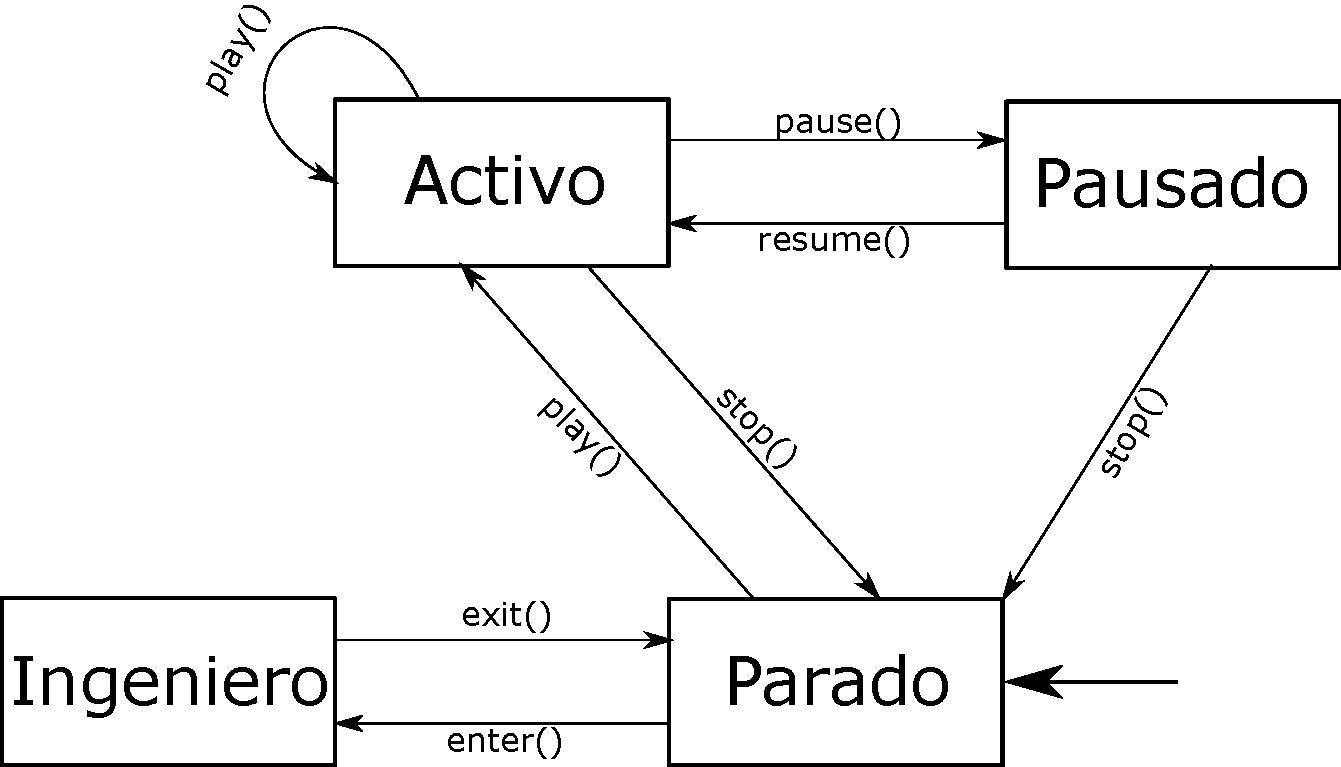
\includegraphics[width=\linewidth/2]{capitulo4/figura4_sched}
		\par\end{centering}
	\smallskip
	\caption{\label{fig:figura4_sched} Diagrama de estados del planificador.}
\end{figure} 

\smallskip

\begin{description}
	\item[Activo] En funcionamiento, reproduciendo activamente una partitura.
	\item[Pausado] No reproduce, mantiene el estado del órgano en el módulo de salida.
	\item[Parado] En espera. Es el estado inicial.
	\item[Ingeniero] Bloqueado, en modo Ingeniería. Ha cedido el control del módulo de salida.
\end{description}

\subsubsection{Algoritmo básico}

Para que todas las pistas se ejecuten simultáneamente, el planificador recorre en cada ciclo todas las listas, avanzando mientras sea el momento de ejecutar el evento correspondiente ($\Delta=0$). Cuando se ha llegado a un evento con $\Delta > 0$ en todas las pistas, se busca el menor valor y se resta a todos los \textit{deltas}. A continuación, se solicita al sistema operativo la espera correspondiente al tiempo restado, y se repite el ciclo. El algoritmo termina cuando todas las pistas han llegado al final.

\begin{algorithmic}
	\LOOP
		\STATE $mindelta \gets \infty$
		\STATE $i\gets 0$
		\WHILE {$i < n_{tracks}$}
			\WHILE {$event_i.delta = 0$ \AND \NOT ($event_i.type = METAEVENT$ \AND \\ $event_i.metaevent.type = END\_OF\_TRACK$)}
				\IF {$event_i.type = NOTE\_ON$}
					\STATE $output\_noteon(i, event_i.param1)$
				\ELSE 
					\IF {$event_i.type = NOTE\_OFF$}
						\STATE $output\_noteoff (i, event_i.param1)$
					\ENDIF
				\ENDIF
				\STATE $event_i \gets event_i.next$
			\ENDWHILE
			\IF {$event_i.delta > 0$ \AND $event_i.delta < mindelta$}
				\STATE $mindelta \gets event_i.delta$
			\ENDIF
		\ENDWHILE
		\STATE $i \gets 0$
		
		\WHILE {$i < n_{tracks}$}
			\STATE $event_i.delta \gets event_i.delta - min$
		\ENDWHILE
		\STATE $sleep (mindelta)$
	\ENDLOOP
\end{algorithmic}

\subsection{Salida hacia la PCB}

El reproductor delega en el módulo de salida las siguientes funciones:

\begin{enumerate}
	\item Dirigir las pistas de \textit{MIDI} al canal de salida correspondiente.
	\item Almacenar el estado de salida (notas pulsadas y no pulsadas).
	\item Volcar la información en el \textit{GPIO}.
\end{enumerate}

Éste será el único módulo que tendremos que cambiar a la hora de pasar de un órgano a otro. El hecho de aislar la salida también nos da flexibilidad para sustituir la interfaz \textit{GPIO} por otro tipo de salida, como la consola, con fines de mantenimiento y depuración.

Las siguientes funciones conforman la interfaz del módulo:

\begin{description}[style=nextline]
	\item[output\_init () : \textit{dword}]
	Inicializa los componentes de la salida. Devuelve 0 en caso de éxito o -1 en caso de error.
	
	\item[output\_destroy ()]
	Cierra el módulo de salida y libera la memoria ocupada.
	
	\item[output\_noteon (track, note)]
	Marcar una nota para activar en el sistema.
	
	\begin{description}
		\item[track : \textit{dword}] Índice de la pista \textit{MIDI}.
		\item[note : \textit{dword}] Número de nota \textit{MIDI}.
	\end{description}
	
	\item[output\_noteon (track, note)]
	Marcar una nota para apagarla en el sistema.
	
	\begin{description}
		\item[track : \textit{dword}] Índice de la pista \textit{MIDI}.
		\item[note : \textit{dword}] Número de nota \textit{MIDI}.
	\end{description}
	
	\item[output\_update ()]
	Vuelca el estado en la salida.
	
	\item[output\_panic ()]
	Vuelve al estado inicial (silenciar todas las notas), y lo vuelca en la salida.
	
	\item[output\_silence ()]
	Silencia todas las notas en la salida, pero mantiene el estado. Útil para pausar la reproducción.
	
\end{description}

\subsubsection{Mapeo de pistas y canales}

Nuestra especificación deja abierta la estructura que pueda tener un archivo MIDI. A pesar de que el sistema podrá descodificar \textit{MIDI} estándar, para lograr una óptima ejecución, la pieza deberá adaptarse a cada órgano concreto.

El módulo de salida permitirá asignar cada pista \textit{MIDI}, que normalmente corresponde a un pentagrama de la partitura, a un canal de salida diferente. La asignación por defecto, para el órgano estudiado, será la siguiente:

\smallskip

\begin{figure}[H]
	\noindent \begin{centering}
		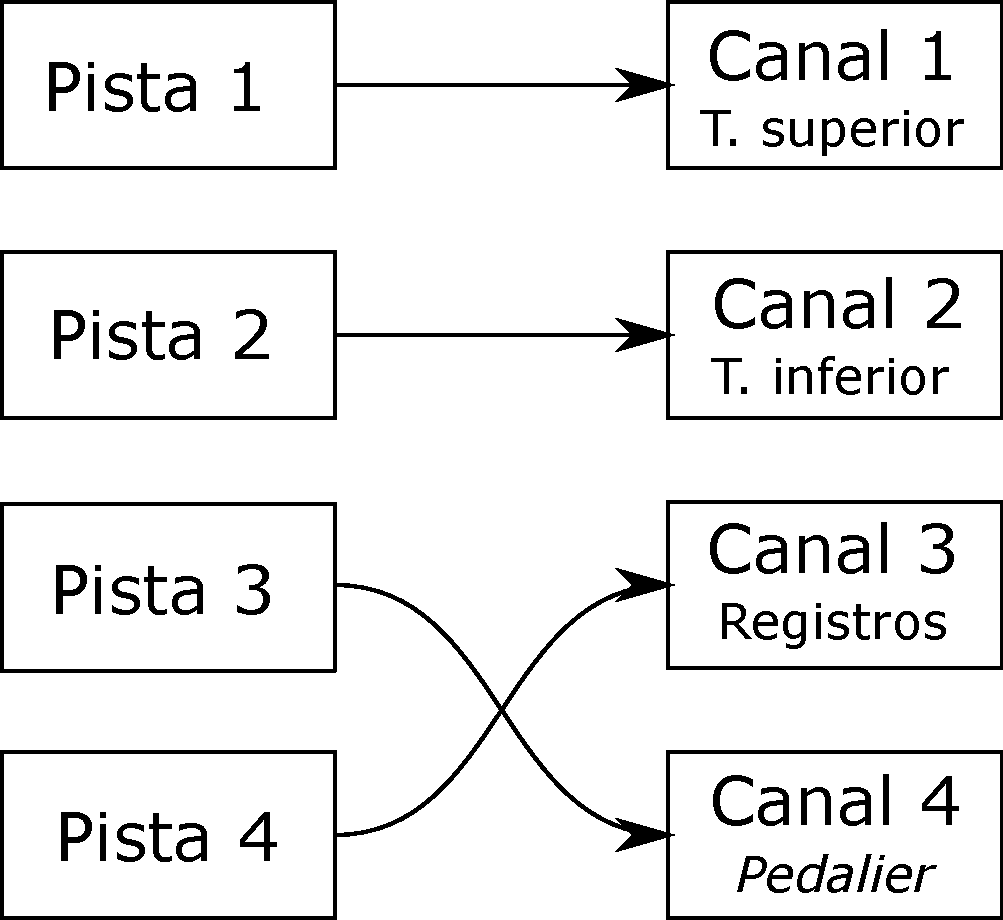
\includegraphics[width=\linewidth/3]{capitulo4/figura4_map}
		\par\end{centering}
	\smallskip
	\caption{\label{fig:figura4_map} Asignación de pistas \textit{MIDI} y canales de salida.}
\end{figure} 

\smallskip

\subsection{Modo Ingeniería}

El sistema requiere un modo de mantenimiento para regular la mecánica, al que se accederá localmente, a través de una interfaz reducida que controlaremos con el codificador rotatorio y el \textit{LCD}.

El codificador permitirá acceder al modo Ingeniería, que detendrá la reproducción ---si estaba en funcionamiento--- y  aislará el planificador, ganando acceso directo a la salida \textit{GPIO}.

Vamos a diseñar la interfaz como una máquina de estados: Inicialmente el modo Ingeniería está desactivado, girando el botón se nos dará la opción de activarlo, y al pulsarlo entraremos en él. Se activará la nota más baja de la primera pista, al girar el botón podremos movernos cíclicamente por todas las notas de esa pista. Pulsando el botón cambiamos a la segunda pista, luego a la tercera, y así hasta la última. Si apretamos nuevamente el botón, volvemos al menú que nos permitirá salir del modo Ingeniería.

Este diagrama muestra las transiciones entre los estados:

\smallskip

\begin{figure}[H]
	\noindent \begin{centering}
		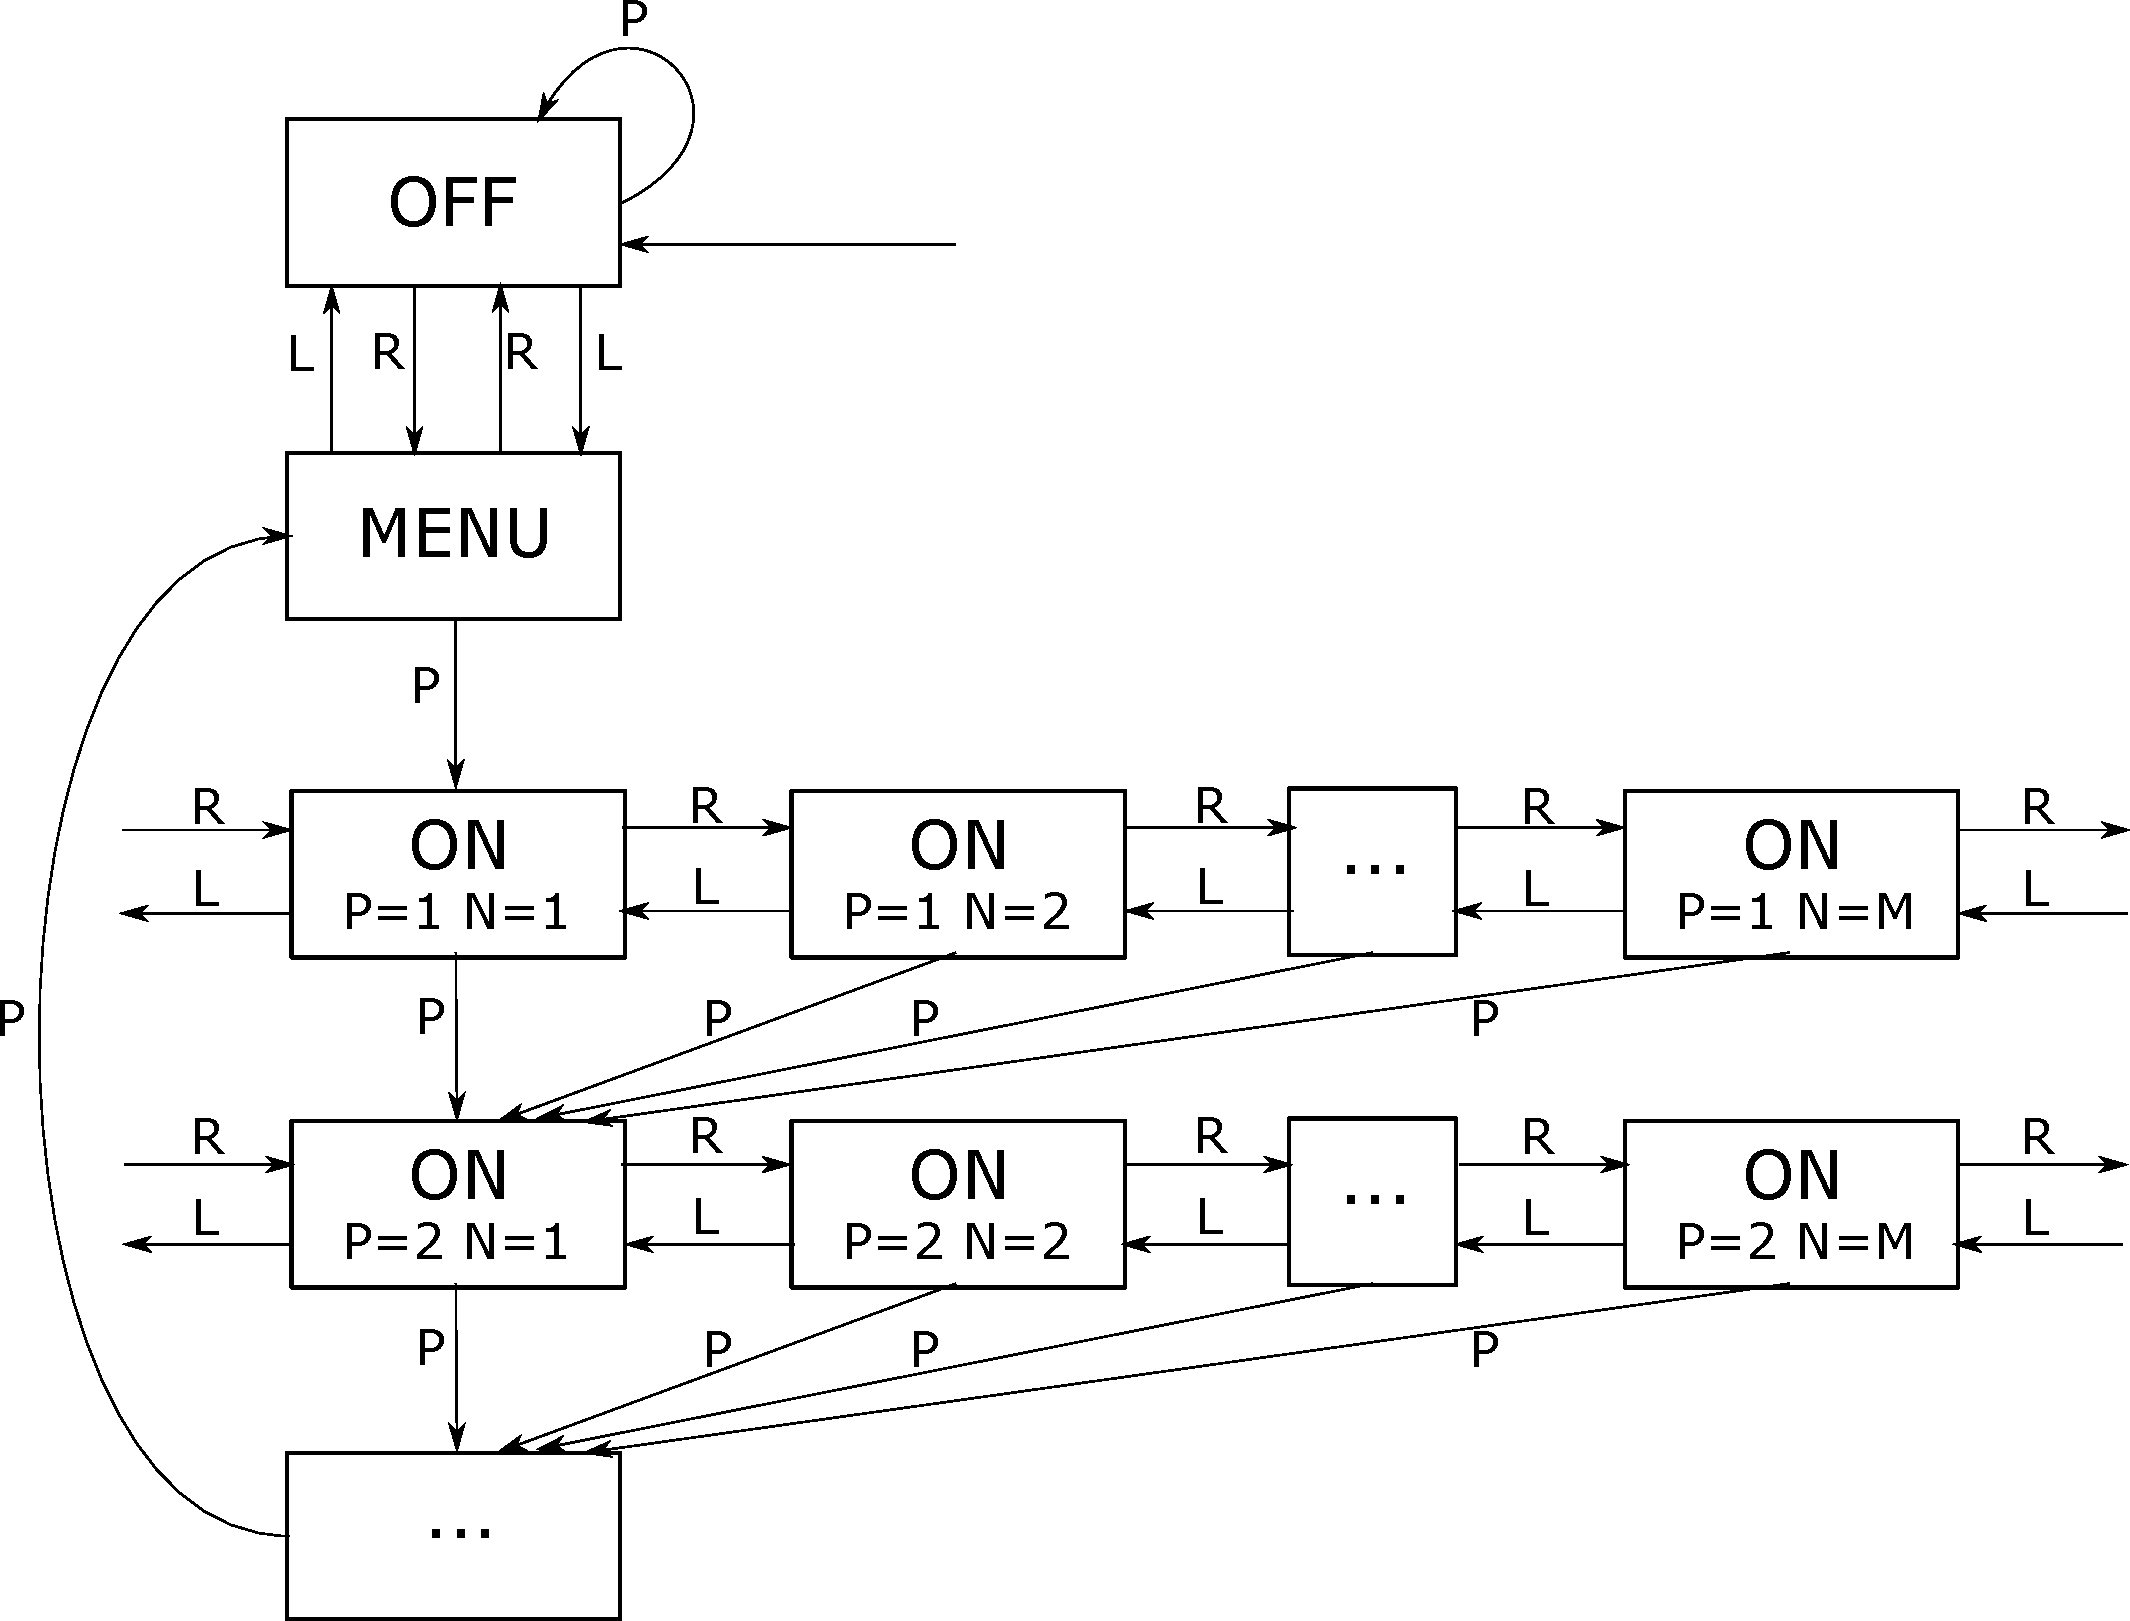
\includegraphics[width=\linewidth*3/4]{capitulo4/figura4_engineer}
		\par\end{centering}
	\smallskip
	\caption{\label{fig:figura4_engineer} Máquina de estados de la interfaz reducida.}
\end{figure} 

\smallskip

\begin{description}
	\item[OFF] Estado inicial, modo Ingeniería apagado. Mostrará el estado del reproductor.
	\item[MENU] Ofrece la opción de entrar en el modo Ingeniería.
	\item[ON] Modo Ingeniería activado, los subestados dependen de la pista y la nota actuales
\end{description}

\subsection{Seguridad}

A pesar de que el acceso al sistema se hará siempre con autentificación de usuario, nos interesa controlar que no todos los usuarios, o no todas las aplicaciones, se conecten al \textit{socket}. La seguridad de \textit{Linux} recae en gran parte sobre su sistema de archivos y permisos. Se creará un nombre de usuario de sistema para ser utilizado exclusivamente por el \textit{socket}, que tendrá permisos de lectura y escritura para dicho usuario y su grupo.

Para autorizar a un usuario a acceder al \textit{socket}, simplemente hay que añadirlo al grupo del usuario propietario.

Por otro lado, el demonio se ejecuta con permisos de \textit{superusuario}, y es inseguro mantenerse durante toda la ejecución con tales privilegios. A pesar de que introduciremos medidas de seguridad en los clientes que desarrollemos para el sistema, reduciremos los permisos después de inicializar el proceso, como medida adicional para evitar problemas.

\section{Base de datos}

La información que queremos almacenar funciona de la siguiente forma:

\begin{enumerate}
	\item Las partituras se guardan en un archivo, cuyo nombre no tiene que coincidir con el título de la partitura.
	\item De una partitura podremos conocer su duración.
	\item Una lista de reproducción es una colección de partituras, y le asignaremos un nombre.
	\item Cada partitura pertenecerá a una lista de reproducción, y solo a una.
	\item Un botón se distingue por su código, y se le asigna a una lista de reproducción, sin perjuicio de que una lista esté asignada a varios botones. Naturalmente, puede haber listas que no estén asignadas a ningún botón.
\end{enumerate}

\subsection{Modelo entidad-relación}

Atendiendo a los requisitos propuestos, modelamos nuestros datos según el siguiente diagrama:

\smallskip

\begin{figure}[H]
	\noindent \begin{centering}
		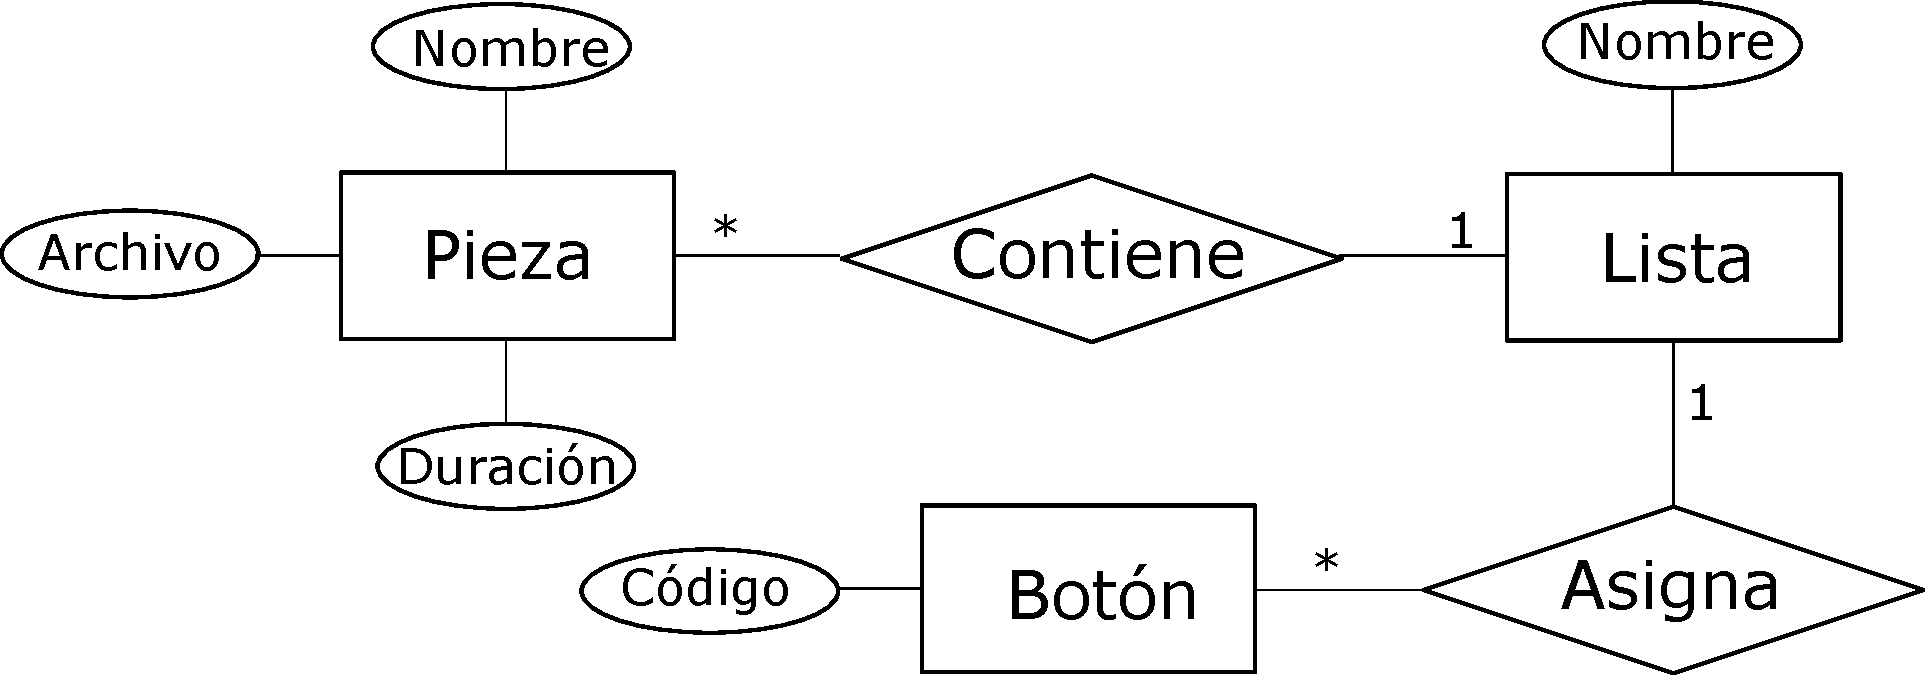
\includegraphics[width=\linewidth*3/4]{capitulo4/figura4_bd_er}
		\par\end{centering}
	\smallskip
	\caption{\label{fig:figura4_bd_er} Modelo entidad-relación.}
\end{figure} 

\smallskip

\subsection{Modelo relacional}

Una vez hemos considerado las entidades, sus atributos y las relaciones, diseñamos el modelo de datos, que depende del tipo de sistema de gestión de bases de datos ---\textit{DBMS (database management system)}--- que vayamos a utilizar. En nuestro caso, utilizaremos un \textit{DBMS} relacional.

\begin{enumerate}
	\item Convertimos en relaciones (tablas) todas las entidades y las relaciones del modelo entidad-relación.
	\item Los atributos de las entidades pasan a ser atributos de las relaciones correspondientes.
	\item Buscamos llaves candidatas y escogemos una como llave primaria. En el caso de Pieza y Lista, no tenemos llave candidata, así que añadimos un ID a cada relación.
	\item Las relaciones Contiene y Asigna tienen cardinalidad N-1, de forma que comparten la clave primaria. Fusionamos Contiene en Pieza y Asigna en Botón.
\end{enumerate}

Una vez hecho esto, el modelo resultante es el siguiente:

\smallskip

\begin{figure}[H]
	\noindent \begin{centering}
		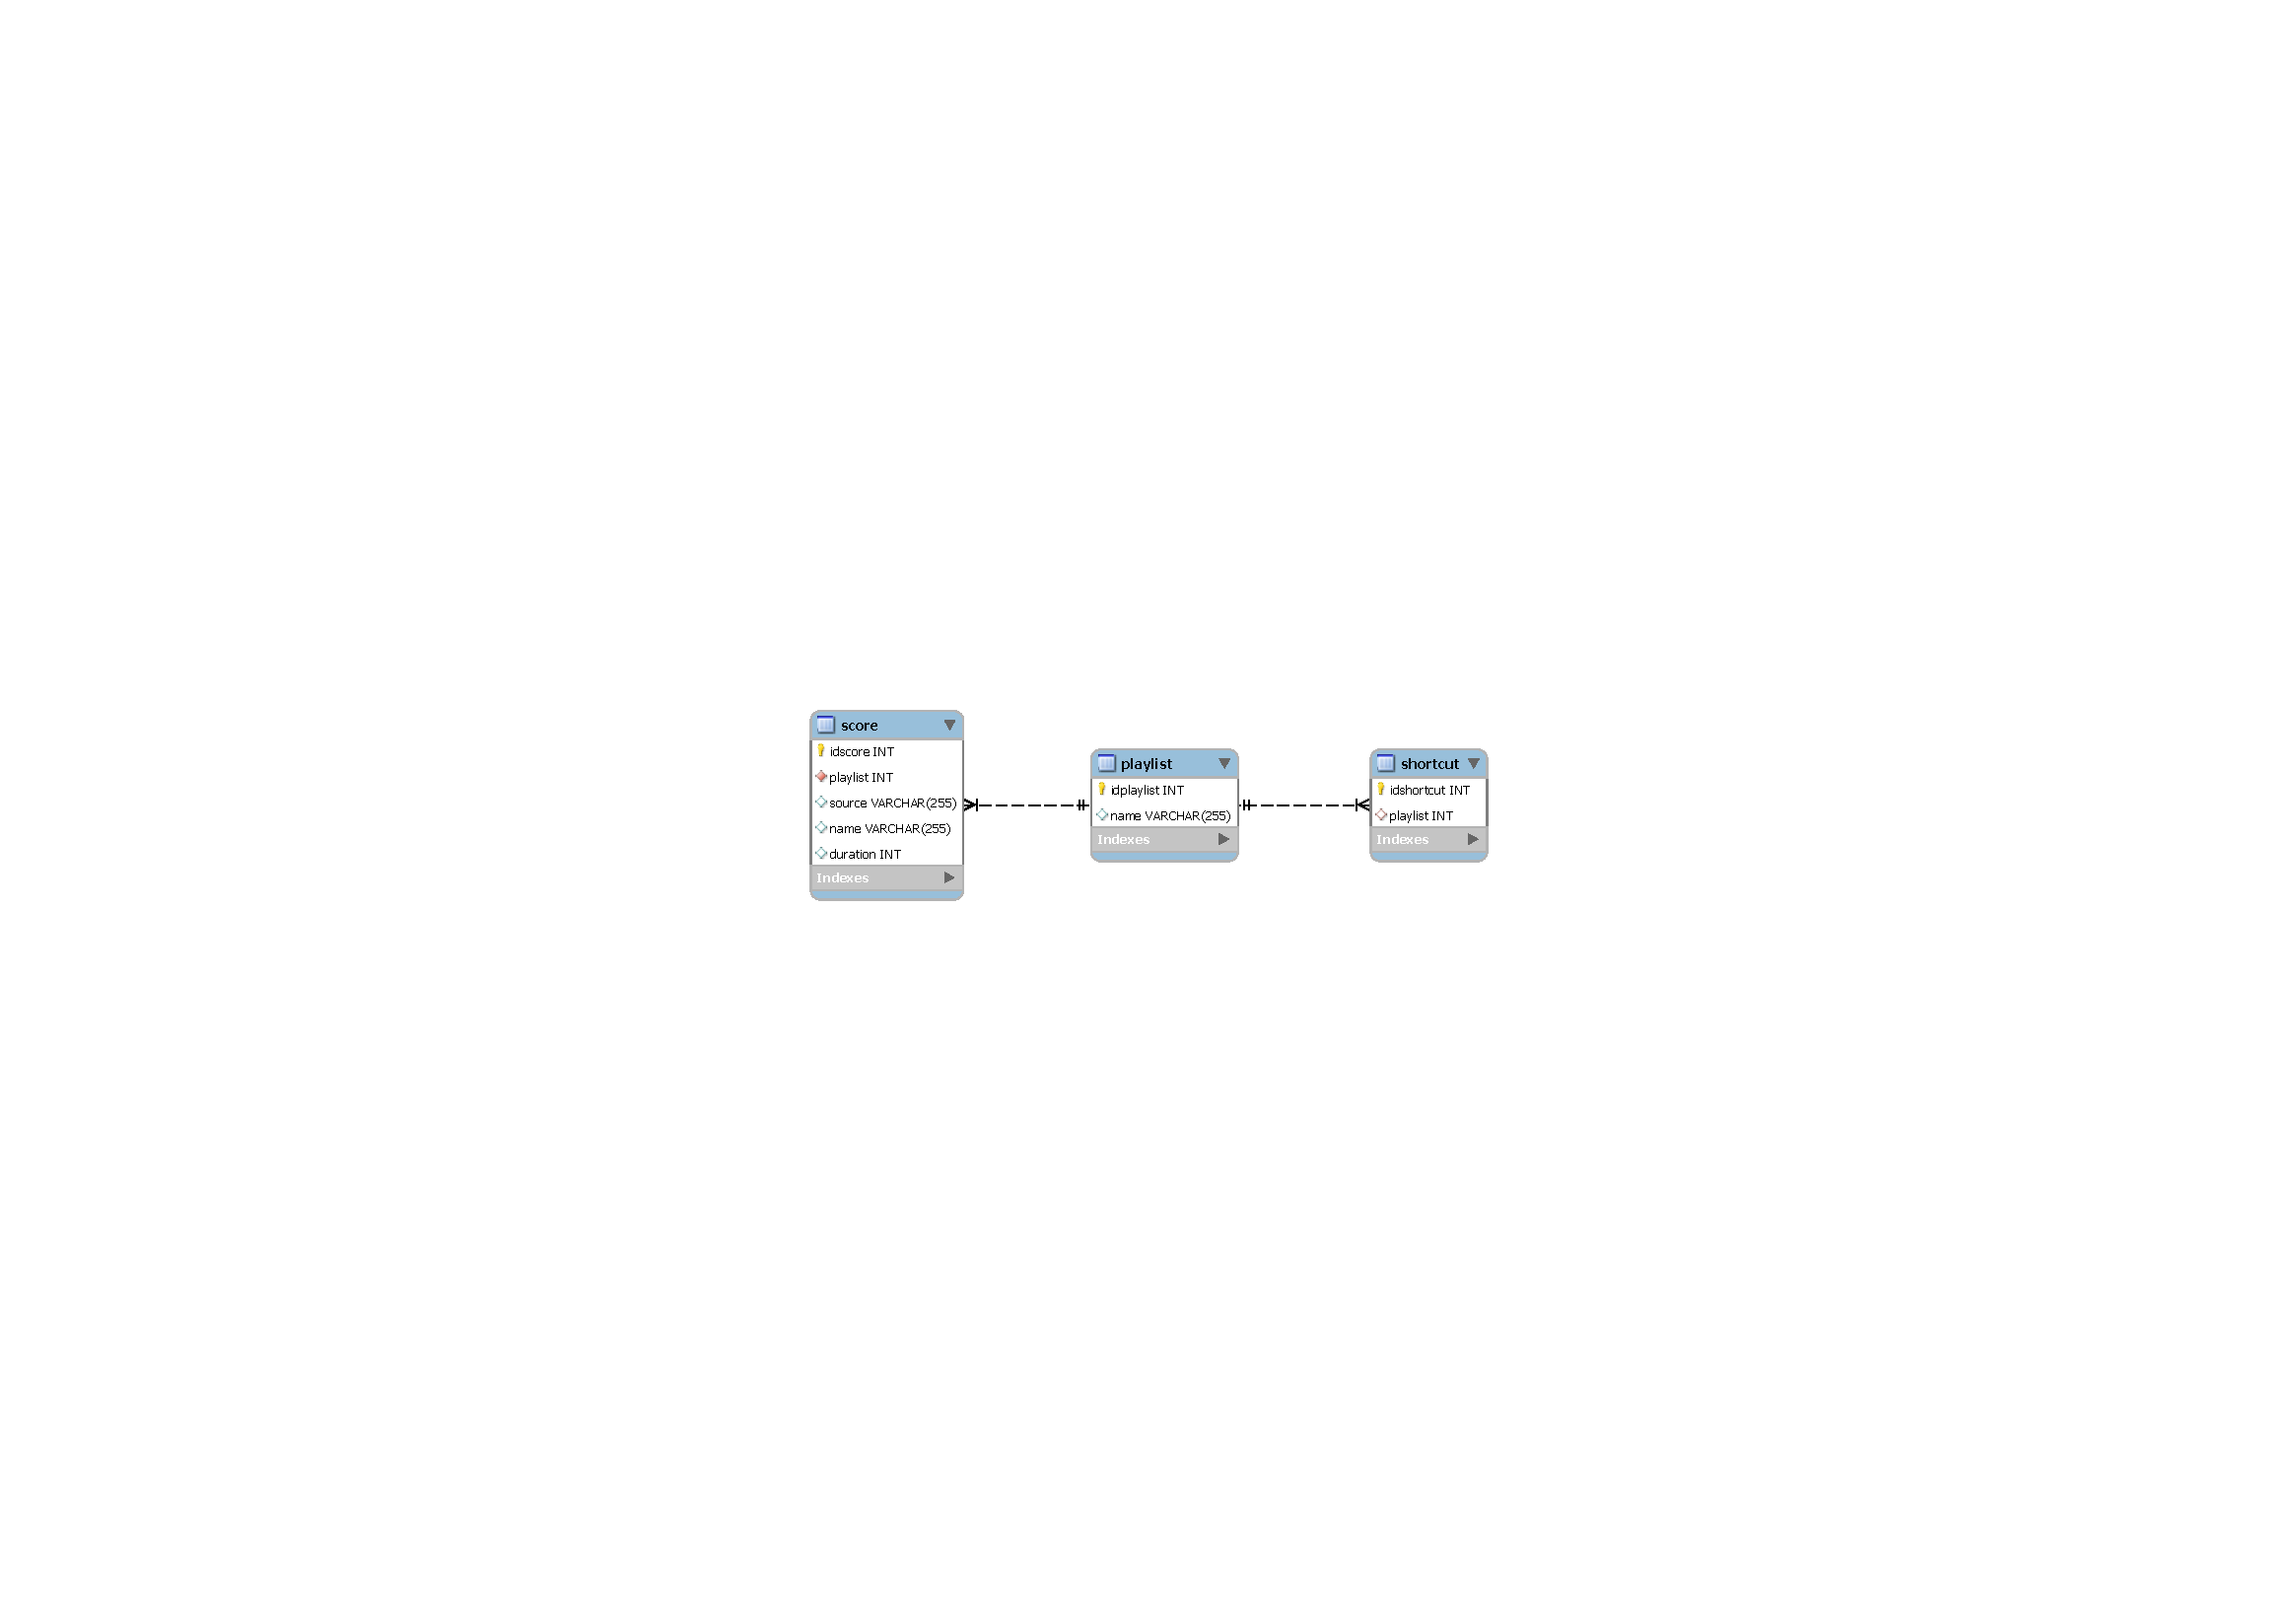
\includegraphics[clip=true, trim=390 340 390 340, width=\linewidth*3/4]{capitulo4/figura4_bd_rel}
		\par\end{centering}
	\smallskip
	\caption{\label{fig:figura4_bd_rel} Modelo relacional.}
\end{figure} 

\smallskip

\subsection{Consistencia}

Para garantizar que la base de datos mantendrá la información coherente y sin anomalías, estudiamos las relaciones para normalizarlas. Podemos verificar que nuestro modelo relacional está en 5ª forma normal, atendiendo a las siguientes condiciones:

\begin{description}
	\item[1FN] El \textit{SGBD} relacional se encarga de que se cumpla la forma normal más básica: las columnas son regulares, no habrá filas duplicadas (por la llave primaria) ni orden alguno entre filas o columnas.
	\item[2FN] Todos los atributos secundarios de cada tabla dependen de la llave primaria, por tanto, está en segunda forma normal.
	\item[3FN] No existen atributos secundarios que dependan transitivamente de la llave primaria, entonces, está en tercera forma normal.
	\item[FNBC] La forma normal de Boyce-Codd establece que los únicos determinantes sean las claves candidatas. Como el modelo está en 3FN y no existen llaves candidatas compuestas, podemos decir que está también en 3FN.
	\item[4FN] La cuarta forma normal extiende la FNBC exigiendo que no existan dependencias multivaluadas no triviales. Este modelo no tiene dependencias multivaluadas, de forma que está en 4FN.
	\item[5FN] Por último, la quinta forma normal especifica que, además de todo lo anterior, cada dependencia de unión sea implicada por claves candidatas. Esto se cumple en nuestro modelo, ya que toda llave externa se vincula a la llave primaria de otra relación.
\end{description}

Nuestro modelo relacional cumple todas las exigencias de las formas normales tenidas en cuenta, con lo que podemos garantizar que el modelo es consistente.

\section{Control remoto}

\subsection{Estilo de la interfaz}

\subsection{Portada}

\subsection{Reproductor}

\subsection{Listas de reproducción}

\subsection{Asignación del mando a listas}

\subsection{Control del usuario}

\subsection{Comunicación con el demonio}

\subsection{Comunicación con la base de datos}

\subsection{Autentificación}

\subsection{Control de energía}

\subsection{Soporte de idiomas}

\section{Aplicaciones auxiliares}

\subsection{Información de archivo MIDI}

\subsection{Comprobación de contraseña}

\subsection{Control de reproducción}

\clearpage{\cleardoublepage}
\clearpage{\pagestyle{empty}\cleardoublepage}